\documentclass[11pt]{article}
\usepackage{url}
\usepackage{latexsym}
\usepackage{graphicx}
\usepackage{amsmath}
\usepackage{cancel}
\usepackage{amsthm}
\usepackage{amssymb}
\usepackage{stmaryrd}


\date{May 6, 2013}
\title{
MKSE312 Final Project
}
\author{
Susan Greenberg and Ayaka Nonaka
}

\begin{document}

\maketitle

\section{Introduction}
In this report, we analyze the Facebook New Orleans dataset (\url{http://socialnetworks.mpi-sws.org/data-wosn2009.html}) using different community detection techniques: modularity maximization using KL algorithm, spectral bipartition, and the Louvain-Twitter algorithm.

We extracted 5 disjoint subgraphs of 2,500 nodes from the dataset to make the computation more feasible.

We were not able to compute the ``flops'' because it is obsolete in recent versions of MATLAB. This article explains more about why that is (near bottom of page): \url{http://www.mathworks.com/company/newsletters/news_notes/clevescorner/winter2000.cleve.html}

\section{Modularity maximization using KL algorithm}
Hopefully we can get some results here...

\section{Spectral bipartition}
Figures \ref{fig:sb1} - \ref{fig:sb5} show the results for spectral bipartition on the 5 subgraphs. The values for $\lambda_2$ for each subgraph respectively are: 0.8992, 0.5614, 0.9856, 0.9116, 0.9352. The $\lambda_2$ values tell us how easily the network can be split into two groups; the smaller the number, the easier to partition.

Subgraph 2 has the smallest $\lambda_2$ (0.5614), suggesting that it is the easiest to split, which seems to make sense since we can identify the two groups in the Figure \ref{fig:sb2}.

On the other hand, subgraph 3 and 5 have the largest $\lambda_2$ (0.9856 and 0.9352 respectively), suggesting that they are the most difficult to split, which also seems to make sense because Figure \ref{fig:sb3} contains some nodes that are highly connected (the long lines that extend throughout the entire plot), and Figure \ref{fig:sb5} shows a cloud of plots that don't seem to have much obvious grouping.

		 \begin{figure}
		 		\begin{center}
		  		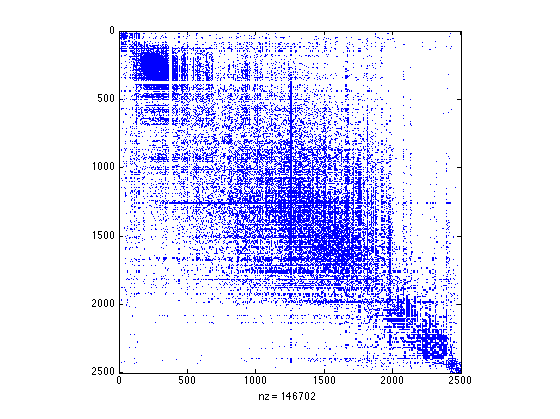
\includegraphics[width=300px]{../graphs/spectral_partition_a1.png}
		  	\end{center}
		  	\caption{Spectral Bipartition for Subgraph 1}
		  	\label{fig:sb1}
		 \end{figure}
		 
		 \begin{figure}
		 		\begin{center}
		  		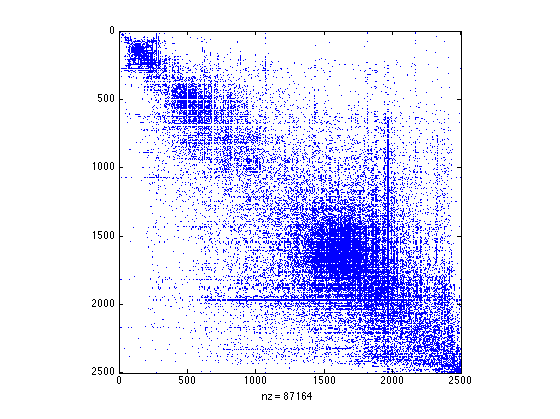
\includegraphics[width=300px]{../graphs/spectral_partition_a2.png}
		  	\end{center}
		  	\caption{Spectral Bipartition for Subgraph 2}
		  	\label{fig:sb2}
		 \end{figure}
		 
		 \begin{figure}
		 		\begin{center}
		  		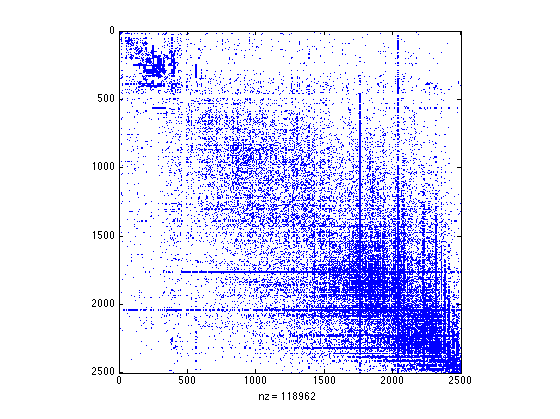
\includegraphics[width=300px]{../graphs/spectral_partition_a3.png}
		  	\end{center}
		  	\caption{Spectral Bipartition for Subgraph 3}
		  	\label{fig:sb3}
		 \end{figure}
		 
		 \begin{figure}
		 		\begin{center}
		  		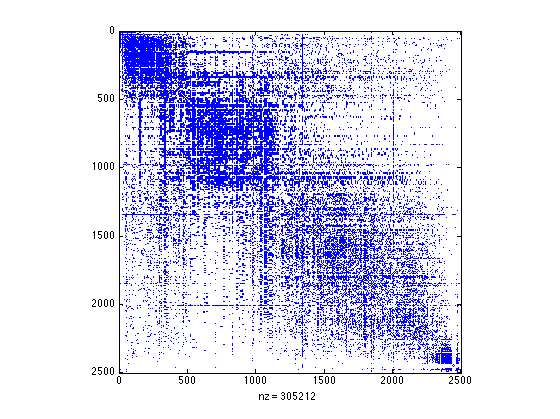
\includegraphics[width=300px]{../graphs/spectral_partition_a4.png}
		  	\end{center}
		  	\caption{Spectral Bipartition for Subgraph 4}
		  	\label{fig:sb4}
		 \end{figure}
		 
		 \begin{figure}
		 		\begin{center}
		  		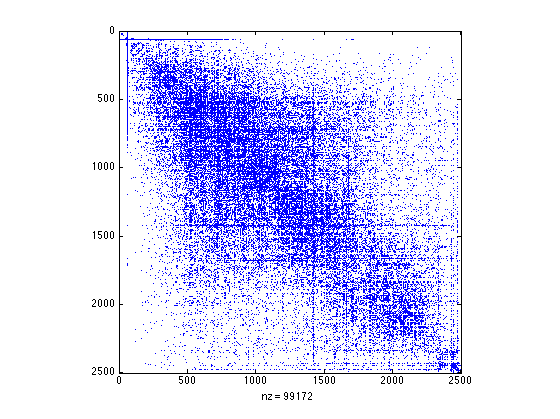
\includegraphics[width=300px]{../graphs/spectral_partition_a5.png}
		  	\end{center}
		  	\caption{Spectral Bipartition for Subgraph 5}
		  	\label{fig:sb5}
		 \end{figure}
		  

\section{Louvain-Twitter algorithm}
We used the Louvain algorithm MATLAB implementation by MIT Strategic Engineering (\url{http://strategic.mit.edu/downloads.php?page=matlab_networks}). We ran the algorithm on the 5 subgraphs. The results are as follows:

\begin{table}[!htbp]
		\begin{tabular}{lll}
		Subgraph & Number of Modules & Modularity \\
	  \hline
		1 & 1134 & 0.0133 \\
		2 & 971 & 0.0287 \\
		3 & 1059 & 0.0179 \\
		4 & 1231 & 0.0057 \\
		5 & 1256 & 0.0204 \\
		\end{tabular}
\end{table}

     
\end{document}
